\documentclass[a3paper,12pt]{extarticle} % Use extarticle for A3 paper size
\usepackage{graphicx} % Include this package for \includegraphics
\usepackage{amsmath}
\usepackage{amssymb} % Include this package for \mathbb
\usepackage[margin=1in]{geometry} % Adjust the margin as needed
\usepackage{placeins} % Include this package for \Floatbarrier

\begin{document}

\author{kipngeno koech - bkoech}
\title{Homework 2 - Introduction to Probabilistic Graphical Models}   
\maketitle

\medskip

\maketitle
\section{Conditional Independence}
\begin{enumerate}
    \item (10 points) State True or False, and briefly justify your answer within 3 lines. The statements are either
    direct consequences of theorems in Koller and Friedman (2009, Ch. 3), or have a short proof. In the
    follows, P is a distribution and G is a BN structure.
    \begin{figure}[h!]
        \centering
        \includegraphics[width=0.5\textwidth]{"conditional_independence.png"}
        \label{fig:example_image}
    \end{figure}
    \\ Recall the definitions of local and global independences of G and independences of P.
    \begin{align}
        I_l(G) &= \{(X \perp \text{NonDescendants}_G(X) \mid \text{Parents}_G(X))\} \\
        I(G) &= \{(X \perp Y \mid Z) : \text{d-separated}_G(X, Y \mid Z)\} \\
        I(P) &= \{(X \perp Y \mid Z) : P(X, Y \mid Z) = P(X \mid Z)P(Y \mid Z)\}
    \end{align}
    \(I_l(G)\) - is the local independence, where a node is independent of its non-descendants given its parents. \(I(G)\) - is the global independence, where two nodes are independent given a set of nodes if they are d-separated. \(I(P)\) - is the independence of a distribution, where two nodes are independent given a set of nodes if the joint distribution factorizes into the product of the marginals.
    \begin{enumerate}
        \item[(a)] In Figure 2, relation 1 is true.
        \\ \textbf{True:} d-separation is a necessary and sufficient condition for conditional independence in a BN. d-separation in G, implies conditional independence in any P that factorizes over G.
        \item[(b)] In Figure 2, relation 2 is true.
        \\ \textbf{True:}  Local independence describe a subset of the conditional independencies that hold in P. 
        \item[(c)] In Figure 2, relation 3 is true.
        \\ \textbf{False:} \(I(G)\) can be a strict subset of \(I(P)\), meaning \(P\) might have additional independencies that are not captured by \(G\), so relation 3 does not always hold.      
        \item[(d)] If G is an I-map for P, then P may have extra conditional independencies than G.
        \\ \textbf{True:} as an I-map only guarantees \(I(G) \subseteq I(P)\), not equality.
        \item[(e)] Two BN structures $G_1$ and $G_2$ are I-equivalent if they have the same skeleton and the same set of v-structures.
        \\ \textbf{True:} Two BN structures are I-equivalent if they have the same set of independencies, which is equivalent to having the same skeleton and the same set of v-structures.
        \item[(f)] If $G_1$ is an I-map of distribution P, and $G_1$ has fewer edges than $G_2$, then $G_2$ is not a minimal I-map of P.
        \\ \textbf{True:} If \(G_1\) is an I-map for \(P\) and has fewer edges than \(G_2\), then \(G_2\) is not minimal, as a minimal I-map has no unnecessary edges.    
        \item[(g)] The P-map of a distribution, if it exists, is unique.
        \\ \textbf{True:} If a perfect map (P-map) for a distribution exists, it is unique.
    \end{enumerate}
\end{enumerate}
\newpage
\section{Exact Inference (Junction Tree a.k.a Clique Tree)}
\begin{enumerate}
    \item Consider the following Bayesian network G:
    \begin{figure}[h!]
        \centering
        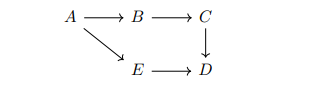
\includegraphics[width=0.5\textwidth]{junction_tree.png}
        \caption{Caption for the image}
        \label{fig:example_image}
    \end{figure}
    \item We are going to construct a junction tree T from G. Please sketch the generated objects in each step.
    \begin{enumerate}
        \item (4 points) Moralize G to construct an undirected graph H.
        \begin{figure}[h!]
            \centering
            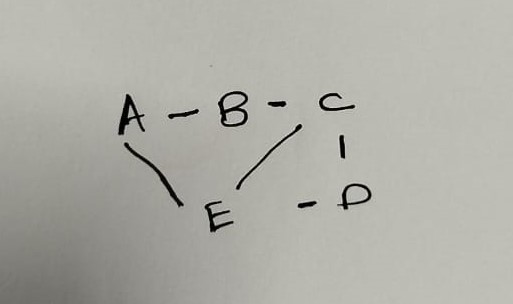
\includegraphics[width=0.5\textwidth]{moralized.jpg}
            \caption{moralized graph}
            \label{fig:example_image}
        \end{figure}
        \\The original graph is moralized by adding edges between the parents who share a common child. For our case node E and C share a common child D, hence an edge is added between E and C.
        \item (7 points) Triangulate H to construct a chordal graph H*.
        (Although there are many ways to triangulate a graph, for the ease of grading, please try adding fewest
        additional edges possible.)
        \begin{figure}[h!]
            \centering
            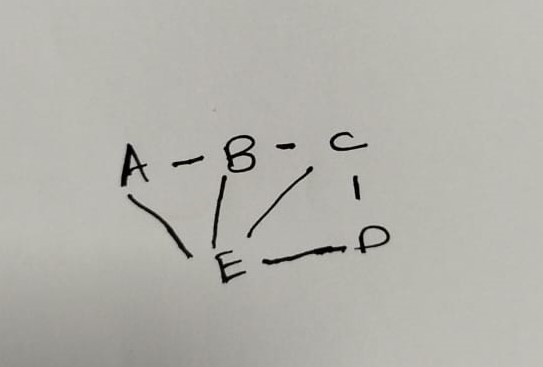
\includegraphics[width=0.5\textwidth]{triangulated.jpg}
            \caption{triangulated graph}
            \label{fig:example_image}
        \end{figure}
        \\The graph is triangulated by adding edges between the nodes that form a triangle with a chord. For our case, the graph is triangulated by adding an edge between B and E, so as to break the chord  formed by the path A-B-C-D-E-A. When we are triangulating a graph, we are ensuring that no cycle of length four or more exists without a chord.
        \item (7 points) Construct a cluster graph U where each node is a maximal clique Ci from H* and each edge is the sepset \(S_{i,j} = C_i \cap C_j\) between adjacent cliques \(C_i\) and \(C_j\).
        \\The maximal cliques are the maximal complete subgraphs of the triangulated graph. The cluster graph is constructed by making each maximal clique a node and adding an edge between two nodes if the corresponding cliques share a variable. The sepset is the intersection of the two cliques.
        \\ The maximal cliques are:
        \begin{itemize}
            \item Clique 1: A, B, E
            \item Clique 2: B, C, E
            \item Clique 3: C, E, D
        \end{itemize}
        The cluster graph is shown in the figure above
        \begin{figure}
            \centering
            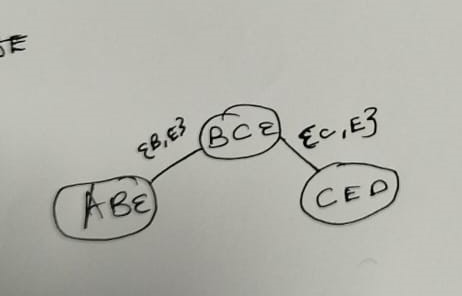
\includegraphics[width=0.5\textwidth]{maximal_clique.jpg}
            \caption{cluster graph}
            \label{fig:example_image}
        \end{figure}
        The edge between the nodes is the sepset between the two cliques. The sepsets are:
        \begin{itemize}
            \item Sepset 1: B, E
            \item Sepset 2: C, E
        \end{itemize}
        \item (7 points) The junction tree T is the maximum spanning tree of U.
        (The cluster graph is small enough to calculate maximum spanning tree in one’s head.)
        \begin{figure}[h!]
            \centering
            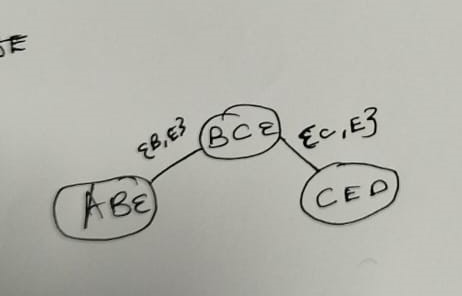
\includegraphics[width=0.5\textwidth]{maximal_clique.jpg}
            \caption{junction tree}
            \label{fig:example_image}
        \end{figure}
        \\The maximum spanning tree is the tree that connects all the nodes in the graph with the minimum possible number of edges. The junction tree is shown in the figure above. It is the same as the cluster graph because the cluster graph is already a tree and each edge has a weight of 2.
    \end{enumerate}

\end{enumerate}
\newpage
\section{Parameter Estimation (HMM - EM Algorithm)}
\begin{enumerate}
    \item Consider an HMM with $T$ time steps, $M$ discrete states, and $K$-dimensional observations as in Figure 3, where $z_t \in \{0, 1\}^M$, $\sum_{s} z_{ts} = 1$, $x_t \in \mathbb{R}^K$ for $t \in [T]$.
    \begin{figure}[h!]
        \centering
        \includegraphics[width=0.5\textwidth]{hmm.png}
        \caption{Caption for the image}
        \label{fig:example_image}
    \end{figure}
\item The joint distribution factorizes over the graph:
\begin{align}
    p(x_{1:T}, z_{1:T}) &= p(z_1) \prod_{t=2}^{T} p(z_t \mid z_{t-1}) \prod_{t=1}^{T} p(x_t \mid z_t). \tag{4}
\end{align}
Now consider the parameterization of CPDs. Let $\pi \in \mathbb{R}^M$ be the initial state distribution and $A \in \mathbb{R}^{M \times M}$ be the transition matrix. The emission density $f(\cdot)$ is parameterized by $\phi_i$ at state $i$. In other words,
\begin{align}
    p(z_{1i} = 1) &= \pi_i, \quad p(z_1) = \prod_{i=1}^{M} \pi_i^{z_{1i}}, \tag{5} \\
    p(z_{tj} = 1 \mid z_{t-1,i} = 1) &= a_{ij}, \quad p(z_t \mid z_{t-1}) = \prod_{i=1}^{M} \prod_{j=1}^{M} a_{ij}^{z_{t-1,i} z_{tj}}, \quad t = 2, \ldots, T, \tag{6} \\
    p(x_t \mid z_{ti} = 1) &= f(x_t; \phi_i), \quad p(x_t \mid z_t) = \prod_{i=1}^{M} f(x_t; \phi_i)^{z_{ti}}, \quad t = 1, \ldots, T. \tag{7}
\end{align}
Let $\theta = (\pi, A, \{\phi_i\}_{i=1}^{M})$ be the set of parameters of the HMM. Given the empirical distribution $\hat{p}$ of $x_{1:T}$, we would like to find the MLE of $\theta$ by solving the following problem:
\begin{align}
    \max_{\theta} \mathbb{E}_{x_{1:T} \sim \hat{p}} [\log p_{\theta}(x_{1:T})]. \tag{8}
\end{align}
However, the marginal likelihood is intractable due to summation over $M^T$ terms:
\begin{align}
    p_{\theta}(x_{1:T}) = \sum_{z_{1:T}} p_{\theta}(x_{1:T}, z_{1:T}). \tag{9}
\end{align}
An alternative is to use the EM algorithm as we saw in the class.
\begin{enumerate}
    \item (10 points) Show that the EM updates can take the following form:
    \begin{align}
        \theta^* &\leftarrow \arg\max_{\theta} \mathbb{E}_{x_{1:T} \sim \hat{p}} [F(x_{1:T}; \theta)] \tag{10}
    \end{align}
    where
    \begin{align}
        F(x_{1:T}; \theta) := &\sum_{i=1}^{M} \gamma(z_{1i}) \log \pi_i + \sum_{t=2}^{T} \sum_{i=1}^{M} \sum_{j=1}^{M} \xi(z_{t-1,i}, z_{tj}) \log a_{ij} \notag \\
        &+ \sum_{t=1}^{T} \sum_{i=1}^{M} \gamma(z_{ti}) \log f(x_t; \phi_i) \tag{11}
    \end{align}
    and $\gamma$ and $\xi$ are the posterior expectations over current parameters $\hat{\theta}$:
    \begin{align}
        \gamma(z_{ti}) &:= \mathbb{E}_{z_{1:T} \sim p_{\hat{\theta}}(z_{1:T} \mid x_{1:T})} [z_{ti}] = p_{\hat{\theta}}(z_{ti} = 1 \mid x_{1:T}), \quad t = 1, \ldots, T \tag{12} \\
        \xi(z_{t-1,i}, z_{tj}) &:= \mathbb{E}_{z_{1:T} \sim p_{\hat{\theta}}(z_{1:T} \mid x_{1:T})} [z_{t-1,i} z_{tj}] = p_{\hat{\theta}}(z_{t-1,i} z_{tj} = 1 \mid x_{1:T}), \quad t = 2, \ldots, T \tag{13}
    \end{align}
    \item (0 points) (No need to answer.) Suppose $\gamma$ and $\xi$ are given, and we use isotropic Gaussian $x_t \mid z_{ti} = 1 \sim \mathcal{N}(\mu_i, \sigma_i^2 I)$ as the emission distribution. Then the parameter updates have the following closed form:
    \begin{align}
        \pi_i^* &\propto \mathbb{E}_{x_{1:T} \sim \hat{p}} [\gamma(z_{1i})] \tag{14} \\
        a_{ij}^* &\propto \mathbb{E}_{x_{1:T} \sim \hat{p}} \left[ \sum_{t=2}^{T} \xi(z_{t-1,i}, z_{tj}) \right] \tag{15} \\
        \mu_{ik}^* &= \frac{\mathbb{E}_{x_{1:T} \sim \hat{p}} \left[ \sum_{t=1}^{T} \gamma(z_{ti}) x_t \right]}{\mathbb{E}_{x_{1:T} \sim \hat{p}} \left[ \sum_{t=1}^{T} \gamma(z_{ti}) \right]} \tag{16} \\
        \sigma_i^{2*} &= \frac{\mathbb{E}_{x_{1:T} \sim \hat{p}} \left[ \sum_{t=1}^{T} \gamma(z_{ti}) \|x_t - \mu_i\|_2^2 \right]}{\mathbb{E}_{x_{1:T} \sim \hat{p}} \left[ \sum_{t=1}^{T} \gamma(z_{ti}) \right] K} \tag{17}
    \end{align}
    \item (10 points) We will use the belief propagation algorithm (Koller and Friedman, 2009, Alg. 10.2) to perform inference for all marginal queries:
    \begin{align}
        \gamma(z_t) &= p_{\hat{\theta}}(z_t \mid x_{1:T}), \quad t = 1, \ldots, T \tag{18} \\
        \xi(z_{t-1}, z_t) &= p_{\hat{\theta}}(z_{t-1}, z_t \mid x_{1:T}), \quad t = 2, \ldots, T \tag{19}
    \end{align}
    For convenience, the notation $\hat{\theta}$ will be omitted from now on. Derive the following BP updates:
    \begin{align}
        \gamma(z_t) &= \frac{1}{Z(x_{1:T})} \cdot s(z_t) \tag{20} \\
        \xi(z_{t-1}, z_t) &= \frac{1}{Z(x_{1:T})} \cdot c(z_{t-1}, z_t) \tag{21}
    \end{align}
    where
    \begin{align}
        s(z_t) &= \alpha(z_t) \beta(z_t), \quad t = 1, \ldots, T \tag{23} \\
        c(z_{t-1}, z_t) &= p(z_t \mid z_{t-1}) p(x_t \mid z_t) \alpha(z_{t-1}) \beta(z_t), \quad t = 2, \ldots, T \tag{24} \\
        Z(x_{1:T}) &= \sum_{z_t} s(z_t) \tag{25}
    \end{align}
    and
    \begin{align}
        \alpha(z_1) &= p(z_1) p(x_1 \mid z_1) \tag{26} \\
        \alpha(z_t) &= p(x_t \mid z_t) \sum_{z_{t-1}} p(z_t \mid z_{t-1}) \alpha(z_{t-1}), \quad t = 2, \ldots, T \tag{27} \\
        \beta(z_{t-1}) &= \sum_{z_t} p(z_t \mid z_{t-1}) p(x_t \mid z_t) \beta(z_t), \quad t = 2, \ldots, T \tag{28} \\
        \beta(z_T) &= 1 \tag{29}
    \end{align}
    \item (0 points) (No need to answer.) Implemented as above, the $(\alpha, \beta)$-recursion is likely to encounter numerical instability due to repeated multiplication of small values. One way to mitigate the numerical issue is to scale $(\alpha, \beta)$ messages at each step $t$, so that the scaled values are always in some appropriate range, while not affecting the inference result for $(\gamma, \xi)$.

    Recall that the forward message is in fact a joint distribution
    \begin{align}
        \alpha(z_t) = p(x_{1:t}, z_t). \tag{30}
    \end{align}
    Define scaled messages by re-normalizing $\alpha$ w.r.t. $z_t$:
    \begin{align}
        \hat{\alpha}(z_t) &= \frac{1}{Z(x_{1:t})} \cdot \alpha(z_t), \tag{31} \\
        Z(x_{1:t}) &= \sum_{z_t} \alpha(z_t). \tag{32}
    \end{align}
    Furthermore, define
    \begin{align}
        r_1 &:= Z(x_1), \tag{33} \\
        r_t &:= \frac{Z(x_{1:t})}{Z(x_{1:t-1})}, \quad t = 2, \ldots, T. \tag{34}
    \end{align}
    Notice that $Z(x_{1:t}) = r_1 \cdot \ldots \cdot r_t$, hence
    \begin{align}
        \hat{\alpha}(z_t) = \frac{1}{r_1 \cdot \ldots \cdot r_t} \cdot \alpha(z_t). \tag{35}
    \end{align}
    Plugging $\hat{\alpha}$ into forward messages, the new $\hat{\alpha}$-recursion is
    \begin{align}
        \hat{\alpha}(z_1) &= \frac{1}{r_1} \cdot p(z_1)p(x_1 \mid z_1), \tag{36} \\
        \hat{\alpha}(z_t) &= \frac{1}{r_t} \cdot p(x_t \mid z_t) \sum_{z_{t-1}} p(z_t \mid z_{t-1}) \hat{\alpha}(z_{t-1}), \quad t = 2, \ldots, T. \tag{37}
    \end{align}
    Since $\hat{\alpha}$ is normalized, each $r_t$ serves as the normalizing constant:
    \begin{align}
        r_t = \sum_{z_t} \tilde{\alpha}(z_t). \tag{38}
    \end{align}
    Now switch focus to $\beta$. In order to make the inference for $(\gamma, \xi)$ invariant of scaling, $\beta$ has to be scaled in a way that counteracts the scaling on $\alpha$. Plugging $\hat{\alpha}$ into the marginal queries,
    \begin{align}
        \gamma(z_t) &= \frac{1}{Z(x_{1:T})} \cdot r_1 \cdot \ldots \cdot r_t \cdot \hat{\alpha}(z_t) \beta(z_t), \tag{39} \\
        \xi(z_{t-1}, z_t) &= \frac{1}{Z(x_{1:T})} \cdot p(z_t \mid z_{t-1}) p(x_t \mid z_t) \cdot r_1 \cdot \ldots \cdot r_{t-1} \cdot \hat{\alpha}(z_{t-1}) \beta(z_t). \tag{40}
    \end{align}
    Since $Z(x_{1:T}) = r_1 \cdot \ldots \cdot r_T$, a natural scaling scheme for $\beta$ is
    \begin{align}
        \hat{\beta}(z_{t-1}) &= \frac{1}{r_t \cdot \ldots \cdot r_T} \cdot \beta(z_{t-1}), \quad t = 2, \ldots, T, \tag{41} \\
        \hat{\beta}(z_T) &:= \beta(z_T). \tag{42}
    \end{align}
    which simplifies the expression for marginals $(\gamma, \xi)$ to
    \begin{align}
        \gamma(z_t) &= \hat{\alpha}(z_t) \hat{\beta}(z_t), \tag{43} \\
        \xi(z_{t-1}, z_t) &= \frac{1}{r_t} \cdot p(z_t \mid z_{t-1}) p(x_t \mid z_t) \hat{\alpha}(z_{t-1}) \hat{\beta}(z_t). \tag{44}
    \end{align}
    The new $\hat{\beta}$-recursion can be obtained by plugging $\hat{\beta}$ into backward messages:
    \begin{align}
        \hat{\beta}(z_{t-1}) &= \frac{1}{r_t} \cdot \sum_{z_t} p(z_t \mid z_{t-1}) p(x_t \mid z_t) \hat{\beta}(z_t), \quad t = 2, \ldots, T, \tag{45} \\
        \hat{\beta}(z_T) &= 1. \tag{46}
    \end{align}
    In other words, $\hat{\beta}(z_{t-1})$ is scaled by $1/r_t$, the normalizer of $\hat{\alpha}(z_t)$.

    The full algorithm is summarized below.

    \textbf{Algorithm 1: Exact inference for $(\gamma, \xi)$}
    \begin{enumerate}
        \item Scaled forward message for $t = 1$:
        \begin{align}
            \tilde{\alpha}(z_1) &= p(z_1)p(x_1 \mid z_1), \tag{47} \\
            r_1 &= \sum_{z_1} \tilde{\alpha}(z_1), \tag{48} \\
            \hat{\alpha}(z_1) &= \frac{1}{r_1} \cdot \tilde{\alpha}(z_1). \tag{49}
        \end{align}
        \item Scaled forward message for $t = 2, \ldots, T$:
        \begin{align}
            \tilde{\alpha}(z_t) &= p(x_t \mid z_t) \sum_{z_{t-1}} p(z_t \mid z_{t-1}) \hat{\alpha}(z_{t-1}), \tag{50} \\
            r_t &= \sum_{z_t} \tilde{\alpha}(z_t), \tag{51} \\
            \hat{\alpha}(z_t) &= \frac{1}{r_t} \cdot \tilde{\alpha}(z_t). \tag{52}
        \end{align}
        \item Scaled backward message for $t = T + 1$:
        \begin{align}
            \hat{\beta}(z_T) = 1. \tag{53}
        \end{align}
        \item Scaled backward message for $t = T, \ldots, 2$:
        \begin{align}
            \hat{\beta}(z_{t-1}) &= \frac{1}{r_t} \cdot \sum_{z_t} p(z_t \mid z_{t-1}) p(x_t \mid z_t) \hat{\beta}(z_t). \tag{54}
        \end{align}
        \item Singleton marginal for $t = 1, \ldots, T$:
        \begin{align}
            \gamma(z_t) = \hat{\alpha}(z_t) \hat{\beta}(z_t). \tag{55}
        \end{align}
        \item Pairwise marginal for $t = 2, \ldots, T$:
        \begin{align}
            \xi(z_{t-1}, z_t) &= \frac{1}{r_t} \cdot p(z_t \mid z_{t-1}) p(x_t \mid z_t) \hat{\alpha}(z_{t-1}) \hat{\beta}(z_t). \tag{56}
        \end{align}

    \end{enumerate}
        \item (15 points) We will implement the EM algorithm (also known as Baum-Welch algorithm), where the E-step performs exact inference and the M-step updates parameter estimates. Please complete the TODO blocks in the provided template \texttt{baum\_welch.py} and submit it to Gradescope. The template contains a toy problem to play with. The submitted code will be tested against randomly generated problem instances.
\end{enumerate}
\end{enumerate}
\newpage
\section{ D-Separation}
\begin{enumerate}
    \item (5 points) Given that the gray nodes are observed, are the variables in A independent to those in B?
    \begin{figure}[h!]
        \centering
        \begin{minipage}{0.48\textwidth}
            \centering
            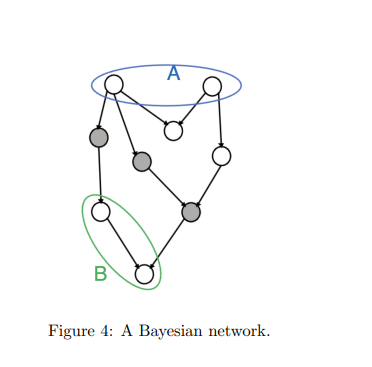
\includegraphics[width=\linewidth]{dseperation_1.png}
            \caption{Unlabeled image}
            \label{fig:example_image1}
        \end{minipage}
        \hfill
        \begin{minipage}{0.48\textwidth}
            \centering
            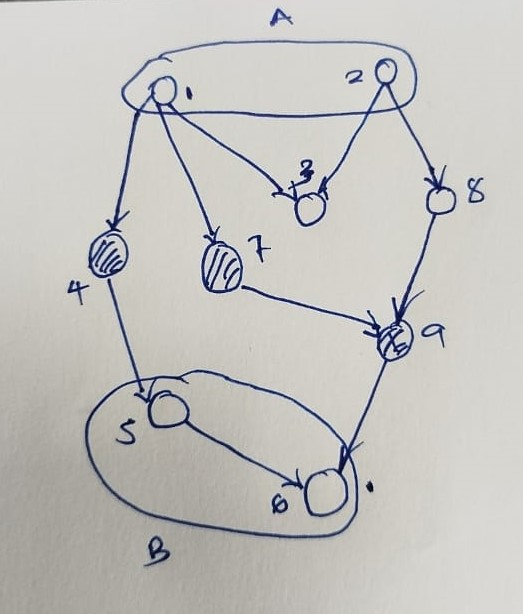
\includegraphics[width=\linewidth]{dseperation_1_labelled.jpg}
            \caption{Labeled image}
            \label{fig:example_image2}
        \end{minipage}
    \end{figure}
    \\
    To check if the variables in A are independent of those in B, we need to check if there is a path between the two sets of variables that is not blocked by any of the observed variables.
    \begin{itemize}
        \item path 1: \(1 \rightarrow 4 \rightarrow 5\) is blocked by 4 because 4 is observed. \(\textbf{(Markov property)}\)
        \item path 2: \(1 \rightarrow 7 \rightarrow 9\) is blocked by 7 because 7 is observed. \(\textbf{(Markov property)}\)
        \item path 3: \(1 \rightarrow 3 \rightarrow 2\) is blocked by 3 because 3 is not observed. \(\textbf{(common effect property)}\)
        \item path 4: \(8 \rightarrow 9 \rightarrow 6\) is blocked by 9 because 9 is  observed. \(\textbf{(Markov property)}\)
    \end{itemize}
    Since all paths are blocked, the variables in A are independent of those in B.
    \item (5 points) Given that the gray nodes are observed, are the nodes 2 and 3 d-separated?
    \begin{figure}[h!]
        \centering
        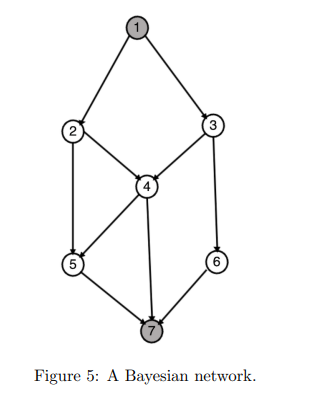
\includegraphics[width=0.5\textwidth]{dseperation_2.png}
        \label{fig:example_image}
    \end{figure}
    \begin{itemize}
        \item path 1: \(2 \rightarrow 1 \rightarrow 3\) is blocked by 1 because 1 is observed. \(\textbf{(common cause property)}\)
        \item path 2: \(2 \rightarrow 4 \rightarrow 3\) is active because 7 which is a child of 4  is observed. \(\textbf{(common effect property)}\)
    \end{itemize}
    Since there is an active path, the nodes 2 and 3 are not d-separated.
    \vspace{22cm}
    \item (5 points) Given that the gray nodes are observed, are the nodes 5 and 6 d-separated?
    \begin{figure}[h!]
        \centering
        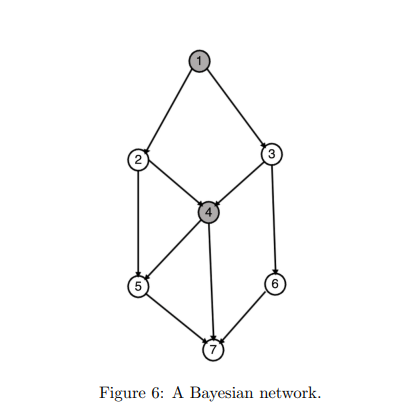
\includegraphics[width=0.5\textwidth]{dseperation_3.png}
        \label{fig:example_image}
    \end{figure} 
    \begin{itemize}
        \item path 1: \(5 \rightarrow 4 \rightarrow 3\) is blocked by 3 because 3 is observed. \(\textbf{(Markov property)}\)
        \item path 2: \(5 \rightarrow 7 \rightarrow 6\) is blocked by 7 because 7 is not observed. \(\textbf{(common effect property)}\)
        \item path 3: \(5 \rightarrow 2 \rightarrow 1 \rightarrow 3 \rightarrow 6\) is blocked by 1 because 1 is observed. \(\textbf{(common cause property)}\)
    \end{itemize}
    Since all paths are blocked, the nodes 5 and 6 are d-separated.
    \item (15 points) Write a python program to check d-separation. Three files have been provided. You have to modify only the \texttt{BN.py} file. The instructions on how to run the code are in the \texttt{check\_dsep.py} file. All the files are provided as a zip file named \texttt{code\_files.zip}.
\end{enumerate}

\end{document}